\documentclass[11pt]{article}
\usepackage[margin=1in]{geometry}
\usepackage[T1]{fontenc}
\usepackage{lmodern}
\usepackage{setspace}
\usepackage{booktabs}
\usepackage{threeparttable}
\usepackage{caption}
\usepackage{amsmath}
\usepackage{pgfplots}
\pgfplotsset{compat=1.17}
\usepackage[hidelinks]{hyperref}
\setstretch{1.3}

\title{Telling Creditors the Whole Story: Integrated Sustainability Reporting and the Cost of Debt\\[0.6em]
\large\textbf{SYNTHETIC TEST PAPER, NOT REAL RESEARCH}}
\author{Synthetic Author\\Fictional Institute of Management, Veldmark}
\date{}

\begin{document}
\maketitle

\begin{abstract}
\noindent Do firms that integrate sustainability information into their annual report borrow more cheaply? We study listed firms in the Republic of Veldmark, where 131 nonfinancial firms voluntarily adopted integrated sustainability reporting for fiscal year 2015. We compare adopters with propensity-matched non-adopters and follow their credit spreads from 2016 to 2019. Propensity score matching addresses endogeneity in the adoption decision, and a Heckman selection model accounts for the fact that spreads are observed only for firms with rated debt. For adopters with propensity scores between 0.1 and 0.9, adoption lowers the credit spread by 31.2 basis points, about 13 percent of the sample mean. Adopters also lengthen the maturity of their debt. The results suggest that creditors price the reduction in information asymmetry that integrated reporting provides.
\end{abstract}

\noindent\textit{Keywords:} integrated reporting; sustainability disclosure; cost of debt; propensity score matching; Heckman selection

\section{Introduction}

Lenders price what they cannot see. A bank or bondholder that is uncertain about a borrower's exposure to environmental liabilities, supply-chain disruptions, or regulatory change will demand compensation for that uncertainty. Firms can reduce it by disclosing more, but sustainability disclosure has long been published in separate reports that are unaudited, inconsistent in scope, and loosely connected to the financial statements. Integrated reporting responds to this problem. An integrated report places sustainability risks and outcomes inside the annual report, ties them to the firm's strategy and financial position, and exposes them to the same board review as the financial accounts.

Whether this matters to creditors is an open question. Research on voluntary disclosure predicts that credible disclosure lowers the cost of capital by reducing information asymmetry and estimation risk. Research on symbolic adoption predicts the opposite: firms adopt reporting frameworks to signal legitimacy while leaving practice unchanged, and sophisticated creditors see through the gesture. Separating these accounts is hard because the firms that choose to adopt integrated reporting differ from those that do not. They are larger, more widely followed by analysts, and more heavily owned by institutions, and each of these traits also predicts cheaper debt.

We study a setting in which a large group of firms adopted integrated reporting at the same time. In 2014 the Veldmark Integrated Reporting Council, a private body chaired by the former exchange president Ilse Marrow, published a reporting framework and invited listed firms to adopt it for fiscal year 2015. Adoption was voluntary. Of 642 nonfinancial firms listed on the Veldmark Exchange at the end of 2014, 131 published an integrated report for fiscal year 2015. We compare these adopters with non-adopters matched on their propensity to adopt and track their credit spreads over the following four years.

Two features of the setting shape our empirical design. First, adoption is a firm choice, so we build a matched comparison group from non-adopters that looked similar to adopters before 2015. Second, the credit spread is observed only for firms with rated public debt, and whether a firm has rated debt is itself a choice that may be related to its cost of borrowing. We therefore estimate the effect of adoption with a Heckman selection model on the matched sample.

We find that, for adopters with propensity scores between 0.1 and 0.9, adoption lowers the credit spread by 31.2 basis points, about 13 percent of the sample mean of 236 basis points. The estimate is similar under entropy balancing and under a simple matching estimator. Adopters also shift toward longer-maturity debt, which is consistent with creditors being more willing to commit capital for longer periods to firms whose risks they understand. The paper contributes to research on disclosure and the cost of capital by showing that the format of sustainability disclosure, and not only its presence, matters to lenders.

\section{Background and Hypotheses}

\subsection{Integrated reporting in Veldmark}

Before 2015, sustainability disclosure in Veldmark was entirely voluntary and fragmented. Most large firms published a stand-alone sustainability report, typically several months after the annual report and with no external assurance. The Council's framework required adopters to do three things: present material sustainability risks in the management commentary of the annual report, connect each risk to a financial line item or strategic objective, and have the board approve the combined document. In practice many adopters also created a board-level sustainability committee to oversee the new content, and some linked a portion of executive pay to sustainability targets reported in the integrated report.

Adopters were concentrated in manufacturing, utilities, and transport, where environmental exposure is high. Examples include Halvorsen Maritime, a coastal shipping firm, and Brekka Cement, the country's second-largest building materials producer. Both had outstanding rated bonds at the time of adoption. Other adopters, such as the software firm Luneby Systems, had no rated debt and borrowed mainly from banks.

\subsection{Hypotheses}

Creditors bear downside risk and care about the tail of the borrower's outcome distribution. Sustainability risks are a large part of that tail for firms with physical assets, long-lived contracts, or regulatory exposure. When these risks are described in a separate, unaudited report, lenders must either invest in their own assessment or apply a generic risk premium. Integrated reporting lowers the cost of assessment and makes the disclosure more credible, because the board approves it alongside audited financial statements and because inconsistencies between the sustainability narrative and the financial accounts become visible. Both mechanisms should reduce the premium that creditors demand.

\medskip
\noindent\textit{Hypothesis 1 (H1).} Adoption of integrated sustainability reporting lowers the firm's cost of debt.
\medskip

The same logic applies to the terms on which creditors lend. Long-maturity debt exposes the lender to more of the borrower's future risk. If integrated reporting makes that risk easier to assess, adopters should be able to borrow at longer maturities.

\medskip
\noindent\textit{Hypothesis 2 (H2).} Adoption of integrated sustainability reporting lengthens the maturity of the firm's debt.
\medskip

\section{Data and Sample}

\subsection{Data sources}

We draw firm financial data from the Veldmark Corporate Filings Database, which contains annual financial statements for all firms listed on the Veldmark Exchange. We identify adopters from the Council's public register, which lists every firm that filed an integrated report for fiscal year 2015, and we confirm each case by reading the annual report. Bond spreads come from the Nordhavn Credit Monitor, which records the yield on each rated bond issued by a Veldmark firm and the yield on the government bond of matching maturity. Board size and CEO pay come from the governance statements filed with the exchange. Delisting dates and reasons come from the exchange's notices.

\subsection{Sample construction}

We begin with the 642 nonfinancial firms listed on the Veldmark Exchange at the end of 2014: 131 adopters and 511 non-adopters. The theory concerns firms that borrow from public and private creditors, and listed firms account for most corporate borrowing in Veldmark, so we treat the exchange population as the population of interest. We restrict the sample to firms with complete data from 2016 to 2019, which gives a balanced panel and ensures that each firm contributes the same number of years. This restriction removes 35 adopters (29 that delisted before the end of 2019 and 6 with missing financial items) and 58 non-adopters (44 delisted and 14 with missing items). The sample for estimating the propensity score therefore contains 549 firms: 96 adopters and 453 non-adopters.

\subsection{Variables}

\textit{Cost of debt.} Our main outcome is the credit spread: the value-weighted average yield on the firm's outstanding rated bonds at the end of each fiscal year, minus the yield on the Veldmark government bond of matching maturity, in basis points. The spread is defined only for firm-years in which the firm has at least one rated bond outstanding.

\textit{Debt maturity.} For H2, we measure maturity as the share of the firm's interest-bearing debt that matures more than three years after the fiscal year end. This measure is available from the notes to the financial statements for every firm-year.

\textit{Adoption.} \textit{Adopt} equals one for firms on the Council's register for fiscal year 2015 and zero otherwise. It does not vary over time within firm.

\textit{Controls.} The outcome equations control for firm size (log of total assets), leverage (total debt over total assets), return on assets, asset tangibility (net property, plant, and equipment over total assets), and interest coverage (operating income over interest expense). All five are measured at the end of fiscal year 2014, before adoption, so that none can be affected by it. All models include industry dummies for the ten Veldmark industry groups and year dummies.

\section{Empirical Strategy}

\subsection{Propensity score and matching}

We estimate the probability of adoption (the propensity score; Rosenbaum and Rubin, 1983) with a logit model on the 549 firms. The model includes log total assets, leverage, return on assets, tangibility, analyst coverage, and institutional ownership, each measured in 2014, together with board size and the log of total CEO pay. Board size and CEO pay are measured in 2016, the first year in which the exchange required a standardized governance statement; earlier disclosures are too inconsistent to code. The model also includes industry dummies. Table~\ref{tab:score} reports the estimates.

Figure~\ref{fig:overlap} shows the distribution of estimated scores for adopters and non-adopters. Many non-adopters have scores near zero and a group of adopters has scores near one. Following Crump et al.\ (2009), we keep only firms with estimated scores between 0.1 and 0.9. This rule removes 31 of the 96 adopters (7 with scores below 0.1 and 24 with scores above 0.9) and 221 of the 453 non-adopters (212 below 0.1 and 9 above 0.9), leaving 65 adopters and 232 non-adopters. Because trimming removes adopters, our estimand is the average effect of adoption on the adopters whose scores lie between 0.1 and 0.9, not on all adopters. Firms that were almost certain to adopt, which tend to be the largest firms on the exchange, are outside the population to which our estimates apply.

Within the trimmed sample we match each adopter to the single nearest non-adopter on the logit of the propensity score, with replacement, within a caliper of 0.2 standard deviations of the logit score (Stuart, 2010). The estimand is the average treatment effect on the treated (ATT). Five adopters have no non-adopter within the caliper and are dropped, leaving 60 matched adopters. They are matched to 52 distinct non-adopters, 8 of which serve as the match for two adopters; these receive a weight of two in all regressions. The remaining 180 trimmed non-adopters are not used. The matched sample thus contains 112 firms and 448 firm-years from 2016 to 2019.

\subsection{Selection into rated debt}

The credit spread exists only for firms with rated bonds, and firms choose whether to issue rated debt. If the unobserved factors that lead a firm to issue rated debt are correlated with its spread, estimates from the rated subsample are biased. We control for selection using Heckman's (1979) two-step procedure. In the first step we estimate a probit model for whether the firm has rated debt outstanding in year $t$ on the full matched sample of 448 firm-years. The selection equation contains the second-stage controls plus year dummies. In the second step we regress the credit spread on \textit{Adopt}, the controls, industry and year dummies, and the inverse Mills ratio ($\lambda$) from the first step.

We estimate the selection equation on the pooled firm-year panel. Because \textit{Adopt} does not vary within firm, our models contain no firm fixed effects, so the pooled correction does not face the incidental-parameters problem that arises with fixed effects in panel selection models (Wooldridge, 1995). Rating status is also stable: 104 of the 112 matched firms have the same status in all four years.

\subsection{Inference}

Adoption is assigned at the firm level, so all standard errors are clustered by firm. The matched sample has 112 firm clusters, and the rated subsample has 71. For the Heckman models, conventional second-stage standard errors ignore that $\lambda$ is itself estimated, so we report standard errors from a firm-cluster bootstrap of both steps (999 replications), resampling firms and re-estimating the probit and the outcome equation in each replication. Clustered standard errors treat the matched sample as fixed. As a check, we also estimate the ATT with a nearest-neighbor matching estimator and compute the Abadie and Imbens (2016) standard error, which accounts for the estimation of the propensity score.

\section{Results}

\subsection{Descriptive statistics}

Table~\ref{tab:desc} reports descriptive statistics for the matched sample. The mean credit spread is 236 basis points. Rated debt is outstanding in 262 of the 448 firm-years (58.5 percent). On average, 54 percent of debt matures in more than three years.

Delisting was more common among adopters than non-adopters. Of the 131 adopters, 29 (22.1 percent) left the exchange before the end of 2019, compared with 44 of the 511 non-adopters (8.6 percent). Most adopter exits followed financial distress: 21 of the 29 were delisted after a missed debt payment or a going-concern opinion from the auditor. Among adopters with rated debt in 2014, those that later delisted had a mean 2014 credit spread of 402 basis points and a mean 2014 interest coverage of 1.4, compared with 231 basis points and 4.1 for adopters that remained listed. Among non-adopters with rated debt in 2014, the corresponding spreads were 298 basis points for firms that later delisted and 246 for firms that remained. Several of the delisted adopters, including Halvorsen Maritime, had cited integrated reporting in their 2015 annual reports as a way to reassure creditors during a period of falling freight rates.

\begin{table}[!htbp]
\centering
\begin{threeparttable}
\caption{Descriptive statistics, matched sample, 2016 to 2019}
\label{tab:desc}
\small
\begin{tabular}{lrrrrr}
\toprule
Variable & N & Mean & SD & Min & Max \\
\midrule
Credit spread (basis points) & 262 & 236.0 & 118.4 & 42.0 & 781.0 \\
Rated debt outstanding (0/1) & 448 & 0.585 & 0.493 & 0 & 1 \\
Debt maturing after 3 years (share) & 448 & 0.540 & 0.210 & 0.020 & 0.980 \\
Adopt (0/1) & 448 & 0.536 & 0.499 & 0 & 1 \\
Log total assets, 2014 & 448 & 7.82 & 1.23 & 4.91 & 11.36 \\
Leverage, 2014 & 448 & 0.289 & 0.142 & 0.012 & 0.744 \\
Return on assets, 2014 & 448 & 0.060 & 0.053 & $-$0.141 & 0.228 \\
Tangibility, 2014 & 448 & 0.346 & 0.178 & 0.018 & 0.861 \\
Interest coverage, 2014 & 448 & 4.62 & 3.37 & $-$1.80 & 19.40 \\
Analyst coverage, 2014 & 448 & 6.26 & 3.99 & 0 & 19 \\
Institutional ownership, 2014 & 448 & 0.464 & 0.190 & 0.041 & 0.912 \\
Board size, 2016 & 448 & 9.46 & 2.15 & 5 & 16 \\
Log CEO pay, 2016 & 448 & 13.89 & 0.62 & 12.21 & 15.64 \\
\bottomrule
\end{tabular}
\begin{tablenotes}\footnotesize
\item Notes: The matched sample contains 60 adopters and 52 distinct matched non-adopters observed annually from 2016 to 2019 (112 firms, 448 firm-years). The credit spread is defined only for firm-years with rated bonds outstanding (262 firm-years from 71 firms). Statistics are unweighted.
\end{tablenotes}
\end{threeparttable}
\end{table}

\subsection{Propensity score and balance}

Table~\ref{tab:score} reports the logit model of adoption. Larger firms, firms with more analyst coverage, and firms with more institutional ownership were more likely to adopt. Firms with larger boards and higher CEO pay were also more likely to adopt, which fits the view that adoption reflects governance capacity. The model's pseudo R-squared is 0.31.

\begin{table}[!htbp]
\centering
\begin{threeparttable}
\caption{Logit model of adoption of integrated reporting (propensity score)}
\label{tab:score}
\small
\begin{tabular}{lc}
\toprule
 & Adopt (0/1) \\
\midrule
Log total assets, 2014 & 0.71*** \\
 & (0.11) \\
Leverage, 2014 & 0.94 \\
 & (0.78) \\
Return on assets, 2014 & 3.10 \\
 & (2.20) \\
Tangibility, 2014 & $-$0.42 \\
 & (0.61) \\
Analyst coverage, 2014 & 0.083*** \\
 & (0.031) \\
Institutional ownership, 2014 & 1.62*** \\
 & (0.58) \\
Board size, 2016 & 0.19*** \\
 & (0.06) \\
Log CEO pay, 2016 & 0.48** \\
 & (0.21) \\
Industry dummies & Yes \\
\midrule
Firms & 549 \\
Adopters & 96 \\
Pseudo R-squared & 0.31 \\
\bottomrule
\end{tabular}
\begin{tablenotes}\footnotesize
\item Notes: Logit coefficients with robust standard errors in parentheses. One observation per firm. *** $p<0.01$, ** $p<0.05$, * $p<0.10$.
\end{tablenotes}
\end{threeparttable}
\end{table}

\begin{figure}[!htbp]
\centering
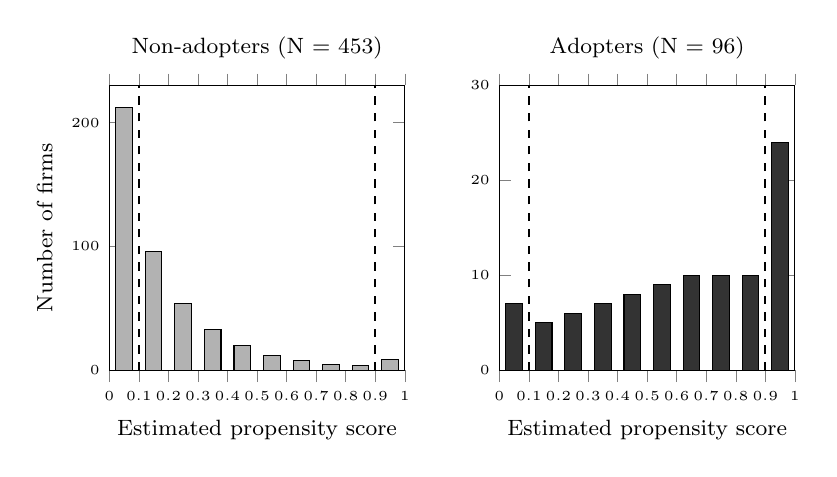
\begin{tikzpicture}
\begin{axis}[
  name=left, width=0.44\textwidth, height=5.2cm,
  ybar, bar width=6pt, bar shift=0pt,
  xmin=0, xmax=1, ymin=0, ymax=230,
  xtick={0,0.1,0.2,0.3,0.4,0.5,0.6,0.7,0.8,0.9,1},
  xticklabel style={font=\tiny, /pgf/number format/fixed},
  yticklabel style={font=\tiny},
  xlabel={\footnotesize Estimated propensity score},
  ylabel={\footnotesize Number of firms},
  title={\footnotesize Non-adopters (N = 453)}]
\addplot[fill=gray!60, draw=black] coordinates {(0.05,212) (0.15,96) (0.25,54) (0.35,33) (0.45,20) (0.55,12) (0.65,8) (0.75,5) (0.85,4) (0.95,9)};
\draw[dashed, thick] (axis cs:0.1,0) -- (axis cs:0.1,230);
\draw[dashed, thick] (axis cs:0.9,0) -- (axis cs:0.9,230);
\end{axis}
\begin{axis}[
  at={(left.east)}, anchor=west, xshift=1.2cm,
  width=0.44\textwidth, height=5.2cm,
  ybar, bar width=6pt, bar shift=0pt,
  xmin=0, xmax=1, ymin=0, ymax=30,
  xtick={0,0.1,0.2,0.3,0.4,0.5,0.6,0.7,0.8,0.9,1},
  xticklabel style={font=\tiny, /pgf/number format/fixed},
  yticklabel style={font=\tiny},
  xlabel={\footnotesize Estimated propensity score},
  title={\footnotesize Adopters (N = 96)}]
\addplot[fill=black!80, draw=black] coordinates {(0.05,7) (0.15,5) (0.25,6) (0.35,7) (0.45,8) (0.55,9) (0.65,10) (0.75,10) (0.85,10) (0.95,24)};
\draw[dashed, thick] (axis cs:0.1,0) -- (axis cs:0.1,30);
\draw[dashed, thick] (axis cs:0.9,0) -- (axis cs:0.9,30);
\end{axis}
\end{tikzpicture}
\caption{Overlap of estimated propensity scores by group. Bars count firms in bins of width 0.1. Dashed lines mark the trimming bounds of 0.1 and 0.9. Trimming removes 7 adopters below 0.1 and 24 above 0.9 (31 in total), and 212 non-adopters below 0.1 and 9 above 0.9 (221 in total). The retained sample has 65 adopters and 232 non-adopters.}
\label{fig:overlap}
\end{figure}

Table~\ref{tab:balance} compares adopters and non-adopters before and after matching. Before matching, adopters are larger, more profitable, more widely covered by analysts, and more heavily owned by institutions, and they have larger boards and higher CEO pay. After matching, no covariate differs significantly between adopters and their matched non-adopters: every p-value exceeds 0.05. We conclude that the matched sample is balanced on all covariates, including leverage. The matched sample contains 60 of the 65 trimmed adopters (5 discarded for lack of a match within the caliper) and 52 of the 232 trimmed non-adopters (180 not used).

\begin{table}[!htbp]
\centering
\begin{threeparttable}
\caption{Covariate balance before and after matching}
\label{tab:balance}
\footnotesize\setlength{\tabcolsep}{4pt}
\begin{tabular}{lccc@{\hspace{1.5em}}ccc}
\toprule
 & \multicolumn{3}{c}{Before matching} & \multicolumn{3}{c}{After matching} \\
\cmidrule(lr){2-4}\cmidrule(lr){5-7}
 & Adopters & Non-adopters & & Adopters & Non-adopters & \\
 & Mean & Mean & p-value & Mean (SD) & Mean (SD) & p-value \\
\midrule
Log total assets, 2014 & 8.34 & 7.12 & $<$0.001 & 7.84 (1.21) & 7.79 (1.25) & 0.824 \\
Leverage, 2014 & 0.301 & 0.268 & 0.081 & 0.312 (0.140) & 0.263 (0.140) & 0.058 \\
Return on assets, 2014 & 0.066 & 0.052 & 0.017 & 0.061 (0.052) & 0.058 (0.055) & 0.759 \\
Tangibility, 2014 & 0.331 & 0.362 & 0.138 & 0.342 (0.181) & 0.351 (0.176) & 0.783 \\
Analyst coverage, 2014 & 8.9 & 4.7 & $<$0.001 & 6.4 (3.9) & 6.1 (4.1) & 0.682 \\
Institutional ownership, 2014 & 0.528 & 0.401 & $<$0.001 & 0.472 (0.188) & 0.455 (0.193) & 0.626 \\
Board size, 2016 & 10.4 & 8.6 & $<$0.001 & 9.6 (2.1) & 9.3 (2.2) & 0.446 \\
Log CEO pay, 2016 & 14.21 & 13.52 & $<$0.001 & 13.92 (0.61) & 13.85 (0.64) & 0.541 \\
\midrule
Firms & 96 & 453 & & 60 & 60 & \\
\bottomrule
\end{tabular}
\begin{tablenotes}\footnotesize
\item Notes: ``Before matching'' uses the 549 firms in the score-estimation sample. ``After matching'' uses the 60 matched adopters and their 60 matches (52 distinct non-adopters; matches used twice are counted twice). p-values are from two-sided t-tests of the difference in means.
\end{tablenotes}
\end{threeparttable}
\end{table}

\subsection{Main results}

Table~\ref{tab:main} reports the main results. Column 1 regresses the credit spread on \textit{Adopt} and the controls in the rated subsample without any selection correction. Adopters' spreads are 24.1 basis points lower ($p<0.05$). Column 2 reports the first-stage probit for having rated debt outstanding. Larger and more leveraged firms are more likely to have rated debt. Adoption has little relation to rated-debt status (coefficient 0.03, standard error 0.08).

Column 3 reports the second stage. Adoption lowers the credit spread by 31.2 basis points ($p<0.01$), about 13 percent of the sample mean of 236 basis points. The inverse Mills ratio is negative and significant ($\lambda = -24.6$, standard error 9.1). Because lambda is significant, selection bias is present, and the estimates in Column 3 are corrected for it. The variance inflation factor for $\lambda$ in Column 3 is 8.7, below the conventional cutoff of 10, so collinearity between the inverse Mills ratio and the second-stage regressors does not threaten the estimates. The corrected estimate is somewhat larger than the uncorrected estimate in Column 1, which suggests that ignoring selection into rated debt understates the benefit of adoption. H1 is supported.

The controls behave as expected. Larger firms and firms with higher interest coverage and profitability pay lower spreads, and more leveraged firms pay higher spreads.

\begin{table}[!htbp]
\centering
\begin{threeparttable}
\caption{Integrated reporting and the credit spread: Heckman selection model}
\label{tab:main}
\small
\begin{tabular}{lccc}
\toprule
 & (1) & (2) & (3) \\
 & OLS, no correction & First stage: probit & Second stage \\
 & Credit spread & Rated debt (0/1) & Credit spread \\
\midrule
Adopt & $-$24.1** & 0.03 & $-$31.2*** \\
 & (9.8) & (0.08) & (10.4) \\
Log total assets, 2014 & $-$17.6*** & 0.412*** & $-$18.3*** \\
 & (4.1) & (0.061) & (4.2) \\
Leverage, 2014 & 131.9*** & 1.18*** & 142.6*** \\
 & (37.5) & (0.42) & (38.9) \\
Return on assets, 2014 & $-$198.7** & 2.04 & $-$210.4** \\
 & (94.2) & (1.31) & (96.1) \\
Tangibility, 2014 & $-$31.8 & 0.55 & $-$35.2 \\
 & (22.4) & (0.37) & (22.8) \\
Interest coverage, 2014 & $-$2.9** & 0.021 & $-$3.1** \\
 & (1.3) & (0.015) & (1.3) \\
Inverse Mills ratio ($\lambda$) & & & $-$24.6*** \\
 & & & (9.1) \\
Industry dummies & Yes & Yes & Yes \\
Year dummies & Yes & Yes & Yes \\
\midrule
Observations (firm-years) & 262 & 448 & 262 \\
Firm clusters & 71 & 112 & 71 \\
R-squared / pseudo R-squared & 0.41 & 0.29 & 0.43 \\
\bottomrule
\end{tabular}
\begin{tablenotes}\footnotesize
\item Notes: Matched sample, 2016 to 2019. Column 2 is estimated on all matched firm-years; Columns 1 and 3 on firm-years with rated bonds outstanding. Non-adopters used as a match twice receive a weight of two. Standard errors in parentheses are clustered by firm; in Columns 2 and 3 they are standard errors from a firm-cluster bootstrap of both steps (999 replications). *** $p<0.01$, ** $p<0.05$, * $p<0.10$.
\end{tablenotes}
\end{threeparttable}
\end{table}

\subsection{Alternative matching and weighting}

Table~\ref{tab:robust} checks whether the main estimate depends on the matching procedure. Column 1 repeats the main estimate. Column 2 replaces nearest-neighbor matching with entropy balancing (Hainmueller, 2012). We reweight the 232 trimmed non-adopters so that the means and variances of the eight score-model covariates and the industry shares match those of the 65 trimmed adopters exactly, and then estimate the same two-step model on the reweighted sample. The largest control weight is 3.9 times the mean control weight, and the effective sample size of the reweighted non-adopters is 164 of 232. Balance holds by construction for the first two moments of these covariates; we make no claim about higher moments or interactions. The estimate is $-29.8$ basis points (standard error 10.9). Column 3 reports the ATT from the nearest-neighbor matching estimator without regression adjustment, computed on firm-level mean spreads for the 31 matched pairs in which both firms have rated debt. The estimate is $-28.7$ basis points, and its Abadie and Imbens (2016) standard error, which accounts for the estimated score, is 11.6. The three estimates agree closely.

\begin{table}[!htbp]
\centering
\begin{threeparttable}
\caption{Alternative matching and weighting procedures}
\label{tab:robust}
\small
\begin{tabular}{lccc}
\toprule
 & (1) & (2) & (3) \\
 & Main (NN matching, & Entropy balancing, & NN matching estimator, \\
 & Heckman) & Heckman & no regression \\
\midrule
Adopt & $-$31.2*** & $-$29.8*** & $-$28.7** \\
 & (10.4) & (10.9) & (11.6) \\
Controls and $\lambda$ & Yes & Yes & No \\
Industry and year dummies & Yes & Yes & No \\
\midrule
Observations & 262 firm-years & 694 firm-years & 31 pairs \\
Firm clusters & 71 & 181 & 62 \\
Estimand & ATT, trimmed & ATT, trimmed & ATT, trimmed \\
\bottomrule
\end{tabular}
\begin{tablenotes}\footnotesize
\item Notes: The outcome is the credit spread in basis points. Column 2 uses the 65 trimmed adopters and 232 entropy-weighted trimmed non-adopters (297 firms; 694 of 1,188 firm-years have rated debt). Column 3 uses firm-level 2016 to 2019 mean spreads. Columns 1 and 2: standard errors from a firm-cluster bootstrap of both steps (999 replications). Column 3: Abadie and Imbens (2016) standard error. *** $p<0.01$, ** $p<0.05$, * $p<0.10$.
\end{tablenotes}
\end{threeparttable}
\end{table}

\subsection{Omitted variables}

A remaining concern is that adopters differ from matched non-adopters on characteristics we do not observe. We assess this concern with coefficient stability. When we drop all controls from the Column 3 specification, keeping only \textit{Adopt}, $\lambda$, and the year dummies, the adoption coefficient is $-44.8$ and the R-squared is 0.09; with the full set of controls, the coefficient is $-31.2$ and the R-squared is 0.43. Following Oster (2019), delta = 2.4, so omitted variable bias is unlikely.

\subsection{Debt maturity}

Table~\ref{tab:maturity} tests H2. Because maturity is observed for every firm-year, no selection correction is needed, and we estimate an OLS regression on all 448 matched firm-years with the same controls and dummies as in Table~\ref{tab:main}. Adoption raises the share of debt maturing after three years by 5.2 percentage points (standard error 1.6, $t = 3.25$), about a tenth of the sample mean of 54 percent. H2 is supported.

We assess the sensitivity of this estimate to an omitted confounder in two ways. First, following Cinelli and Hazlett (2020), the partial R-squared of \textit{Adopt} with the outcome is 0.024. The robustness value for reducing the estimate to zero is 0.145, and the robustness value for making it insignificant at the 5 percent level is 0.060, computed from $t = 3.25$ and 429 residual degrees of freedom. A confounder would have to explain at least 6.0 percent of the residual variance of both adoption and maturity to make the estimate insignificant. For comparison, leverage, the observed covariate most strongly related to maturity, explains 0.4 percent of the residual variance of adoption and 1.8 percent of the residual variance of maturity. A confounder three times as strong as leverage (1.2 and 5.4 percent) would therefore not make the estimate insignificant. This benchmarking assumes that the omitted confounder is no more than three times as strongly related to adoption and maturity as leverage is. Second, following Frank (2000), the impact threshold of a confounding variable (ITCV) is 0.067: an omitted variable would need a correlation of about 0.26 with both adoption and maturity, conditional on the controls, to make the estimate insignificant at the 5 percent level. The largest impact of any observed covariate, computed as the product of its partial correlations with adoption and maturity, is 0.0085 (leverage: $0.063 \times 0.134$). Both analyses rest on the assumption that the observed covariates are a reasonable guide to the strength of an unobserved one, and neither shows that no such confounder exists.

\begin{table}[!htbp]
\centering
\begin{threeparttable}
\caption{Integrated reporting and debt maturity (H2)}
\label{tab:maturity}
\small
\begin{tabular}{lc}
\toprule
 & Debt maturing after 3 years (share) \\
\midrule
Adopt & 0.052*** \\
 & (0.016) \\
Controls (2014) & Yes \\
Industry and year dummies & Yes \\
\midrule
Observations (firm-years) & 448 \\
Firm clusters & 112 \\
R-squared & 0.27 \\
\midrule
\multicolumn{2}{l}{\textit{Sensitivity to an omitted confounder}} \\
Partial R-squared of Adopt with outcome & 0.024 \\
Robustness value, $q=1$ & 0.145 \\
Robustness value, $q=1$, $\alpha=0.05$ & 0.060 \\
ITCV & 0.067 \\
Largest observed impact (leverage) & 0.0085 \\
\bottomrule
\end{tabular}
\begin{tablenotes}\footnotesize
\item Notes: OLS on the matched sample, 2016 to 2019. Non-adopters used as a match twice receive a weight of two. Standard errors clustered by firm in parentheses. Robustness values follow Cinelli and Hazlett (2020) and use the model's $t$-statistic and 429 residual degrees of freedom. *** $p<0.01$, ** $p<0.05$, * $p<0.10$.
\end{tablenotes}
\end{threeparttable}
\end{table}

\section{Threats to Validity}

Three limitations deserve mention. First, credit spreads measure the cost of public debt only. Adopters that borrow mainly from banks, such as Luneby Systems, are absent from the spread analysis, and bank loan pricing may respond differently to disclosure. The Heckman correction addresses the resulting sample selection, but we cannot observe private loan terms directly.

Second, our spread measure uses year-end yields. Bond prices move with market conditions, and year-end yields may be noisy measures of a firm's cost of borrowing over the year. Noise in the outcome should reduce precision rather than bias the estimates, and our standard errors remain small enough to reject the null.

Third, Veldmark is a small, bank-oriented economy, and the Council's framework differs in detail from frameworks used elsewhere. The size of the effect may not carry over to larger bond markets where sustainability information is more widely produced by rating agencies and data vendors.

\section{Discussion and Conclusion}

Integrated reporting is often dismissed as a relabeling of existing disclosure. Our evidence suggests that creditors disagree. Firms that adopted the Veldmark framework in 2015 and had propensity scores between 0.1 and 0.9 paid about 31 basis points less on their rated bonds over the following four years than matched non-adopters, and they shifted toward longer-maturity debt. The estimates are similar under nearest-neighbor matching, entropy balancing, and a simple matching estimator.

These findings have implications for managers and regulators. For managers, the savings are large relative to the cost of preparing an integrated report: for a firm with the sample median of 1.9 billion Veldmark crowns in rated bonds, a 31 basis point reduction is worth about 5.9 million crowns a year. For regulators considering whether to mandate integrated reporting, our results suggest that the benefits of credible sustainability disclosure accrue in part through the debt market.

The study also points to questions for future work. We cannot say which part of the integrated report creditors respond to: the content, the board's approval, or the link to financial statements. Nor can we say whether the effect persists once integrated reporting becomes common and no longer distinguishes adopters from other firms. Later waves of adoption in Veldmark may allow these questions to be answered.

\section*{References}
\small
\begin{description}\setlength{\itemsep}{2pt}
\item Abadie, A., and Imbens, G. W. (2016). Matching on the estimated propensity score. \textit{Econometrica}, 84(2), 781--807.
\item Cinelli, C., and Hazlett, C. (2020). Making sense of sensitivity: Extending omitted variable bias. \textit{Journal of the Royal Statistical Society Series B}, 82(1), 39--67.
\item Crump, R. K., Hotz, V. J., Imbens, G. W., and Mitnik, O. A. (2009). Dealing with limited overlap in estimation of average treatment effects. \textit{Biometrika}, 96(1), 187--199.
\item Frank, K. A. (2000). Impact of a confounding variable on a regression coefficient. \textit{Sociological Methods and Research}, 29(2), 147--194.
\item Hainmueller, J. (2012). Entropy balancing for causal effects. \textit{Political Analysis}, 20(1), 25--46.
\item Heckman, J. J. (1979). Sample selection bias as a specification error. \textit{Econometrica}, 47(1), 153--161.
\item Oster, E. (2019). Unobservable selection and coefficient stability: Theory and evidence. \textit{Journal of Business and Economic Statistics}, 37(2), 187--204.
\item Rosenbaum, P. R., and Rubin, D. B. (1983). The central role of the propensity score in observational studies for causal effects. \textit{Biometrika}, 70(1), 41--55.
\item Stuart, E. A. (2010). Matching methods for causal inference: A review and a look forward. \textit{Statistical Science}, 25(1), 1--21.
\item Wooldridge, J. M. (1995). Selection corrections for panel data models under conditional mean independence assumptions. \textit{Journal of Econometrics}, 68(1), 115--132.
\end{description}

\end{document}
